%
\documentclass[11pt, oneside]{article}      % use 'amsart' instead of 'article' for AMSLaTeX format
\usepackage{geometry}                       % See geometry.pdf to learn the layout options. There are lots.
\geometry{letterpaper}                      % ... or a4paper or a5paper or ...
%\geometry{landscape}                       % Activate for for rotated page geometry
\usepackage[parfill]{parskip}               % Activate to begin paragraphs with an empty line rather than an indent
\usepackage{graphicx}                       % Use pdf, png, jpg, or eps with pdflatex; use eps in DVI mode
                                            % TeX will automatically convert eps --> pdf in pdflatex
\usepackage{amssymb}
%\date{\today}                              % Activate to display a given date or no date
\title{Structure of the port-Hamiltonian system\\\texttt{ThieleSmall}}
%
\usepackage{authblk}
\usepackage{hyperref}
%\renewcommand\Authands{ and }
%
%
\author[1]{The \textsc{PyPHS}\footnote{\url{https://github.com/afalaize/pyphs}} development team}
%
\affil[1]{Project-team S3\footnote{\url{http://s3.ircam.fr}}\\STMS, IRCAM-CNRS-UPMC (UMR 9912)\\1 Place Igor-Stravinsky, 75004 Paris, France}
%
\begin{document}
%
\maketitle
%
%
\section{System netlist}
%
%
\begin{center}
%
\texttt{
\begin{tabular}{llllll}
\hline
line & label & dictionary.component & nodes &     parameters \\ \hline
%
$\ell_1$ & IN & electronics.source & ('A', 'ref') & $\left\{ 
%
\begin{tabular}{ll}
%
type & voltage
\\
\end{tabular}\right.$
 \\
$\ell_2$ & R & electronics.resistor & ('A', 'B') & $\left\{ 
%
\begin{tabular}{ll}
%
R & ('R', 1000.0)
\\
\end{tabular}\right.$
 \\
$\ell_3$ & L & electronics.inductor & ('B', 'C') & $\left\{ 
%
\begin{tabular}{ll}
%
L & ('L', 0.05)
\\
\end{tabular}\right.$
 \\
$\ell_4$ & G & connectors.gyrator & ('C', 'ref', 'D', 'ref') & $\left\{ 
%
\begin{tabular}{ll}
%
alpha & ('Bl', 50)
\\
\end{tabular}\right.$
 \\
$\ell_5$ & M & mechanics.mass & ('D', 'E') & $\left\{ 
%
\begin{tabular}{ll}
%
M & ('M', 0.1)
\\
\end{tabular}\right.$
 \\
$\ell_6$ & K & mechanics.springcubic & ('E', 'F') & $\left\{ 
%
\begin{tabular}{ll}
%
K2 & ('K2', 1e+20)
\\
K0 & ('K0', 5000.0)
\\
\end{tabular}\right.$
 \\
$\ell_7$ & A & mechanics.damper & ('F', 'ref') & $\left\{ 
%
\begin{tabular}{ll}
%
A & ('A', 1)
\\
\end{tabular}\right.$
 \\
\hline
\end{tabular}
%
}
%
\end{center}
%
    %
    \begin{figure}[!h]
    \begin{center}
    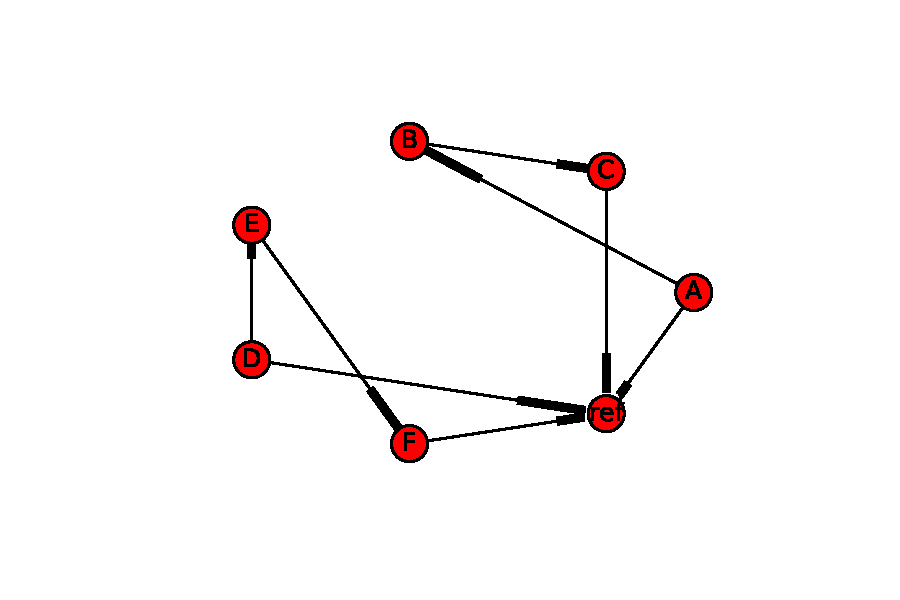
\includegraphics[width=\linewidth]{/Users/Falaize/Documents/DEV/python/pyphs/pyphs/tests/ThieleSmall/figures/ThieleSmall_graph.pdf}
    %
    \caption{\label{fig:graph_ThieleSmall} Graph of system \texttt{ThieleSmall}. }
    \end{center}
    \end{figure}
    %\section{System dimensions}
%
$\dim(\mathbf{x})=$ $ n_\mathbf{x} = 3 ; $ 
%
\\
%
$\dim(\mathbf{w})=$ $ n_\mathbf{w} = 2 ; $ 
%
\\
%
$\dim(\mathbf{y})=$ $ n_\mathbf{y} = 1 ; $ 
%
\\
%
$\dim(\mathbf{p})=$ $ n_\mathbf{p} = 0 ; $ 
%
\\
%
%
\section{System variables}
%
State variable $ \mathbf{x} = \left(\begin{array}{c}x_{\mathrm{M}}\\x_{\mathrm{L}}\\x_{\mathrm{K}}\end{array}\right) ; $ 
%
\\
%
Dissipation variable $ \mathbf{w} = \left(\begin{array}{c}w_{\mathrm{R}}\\w_{\mathrm{A}}\end{array}\right) ; $ 
%
\\
%
Input $ \mathbf{u} = \left(\begin{array}{c}u_{\mathrm{IN}}\end{array}\right) ; $ 
%
\\
%
Output $ \mathbf{y} = \left(\begin{array}{c}y_{\mathrm{IN}}\end{array}\right) ; $ 
%
\\
%
%
\section{Constitutive relations}
%
Hamiltonian $ \mathtt{H}(\mathbf{x}) = \frac{\mathrm{K0}}{2} \cdot x_{\mathrm{K}} \cdot \left(\frac{x_{\mathrm{K}}^{3}}{2} + x_{\mathrm{K}}\right) + \frac{0.5}{\mathrm{M}} \cdot x_{\mathrm{M}}^{2} + \frac{0.5}{\mathrm{L}} \cdot x_{\mathrm{L}}^{2} ; $ 
%
\\
%
Hamiltonian gradient $ \nabla \mathtt{H}(\mathbf{x}) = \left(\begin{array}{c}\frac{1.0}{\mathrm{M}} \cdot x_{\mathrm{M}}\\\frac{1.0}{\mathrm{L}} \cdot x_{\mathrm{L}}\\\frac{\mathrm{K0}}{2} \cdot x_{\mathrm{K}} \cdot \left(\frac{3}{2} \cdot x_{\mathrm{K}}^{2} + 1\right) + \frac{\mathrm{K0}}{2} \cdot \left(\frac{x_{\mathrm{K}}^{3}}{2} + x_{\mathrm{K}}\right)\end{array}\right) ; $ 
%
\\
%
Dissipation function $ \mathbf{z}(\mathbf{w}) = \left(\begin{array}{c}\mathrm{R} \cdot w_{\mathrm{R}}\\\mathrm{A} \cdot w_{\mathrm{A}}\end{array}\right) ; $ 
%
\\
%
Jacobian of dissipation function $ \mathcal{J}_{\mathbf{z}}(\mathbf{w}) = \left(\begin{array}{cc}\mathrm{R} & 0\\0 & \mathrm{A}\end{array}\right) ; $ 
%
\\
%
%
\section{System parameters}
%
%
\subsection{Constant}
%
\begin{center}
%
\begin{tabular}{ll}
%
\hline
parameter & value (SI)
\\ \hline
Bl :& 50
\\
K2 :& 1e+20
\\
R :& 1000.0
\\
K0 :& 5000.0
\\
L :& 0.05
\\
A :& 1
\\
M :& 0.1
\\
\hline
\end{tabular}
%
\end{center}
%
\section{System structure}
%

%
$ \mathbf{M} = \left(\begin{array}{cccccc}0 & 1.0 \cdot \mathrm{Bl} & -1.0 & 0 & -1.0 & 0\\- 1.0 \cdot \mathrm{Bl} & 0 & 0 & -1.0 & 0 & 1.0\\1.0 & 0 & 0 & 0 & 0 & 0\\0 & 1.0 & 0 & 0 & 0 & 0\\1.0 & 0 & 0 & 0 & 0 & 0\\0 & -1.0 & 0 & 0 & 0 & 0\end{array}\right) ; $ 
%
\\
%
$ \mathbf{M_{xx}} = \left(\begin{array}{ccc}0 & 1.0 \cdot \mathrm{Bl} & -1.0\\- 1.0 \cdot \mathrm{Bl} & 0 & 0\\1.0 & 0 & 0\end{array}\right) ; $ 
%
\\
%
$ \mathbf{M_{xw}} = \left(\begin{array}{cc}0 & -1.0\\-1.0 & 0\\0 & 0\end{array}\right) ; $ 
%
\\
%
$ \mathbf{M_{xy}} = \left(\begin{array}{c}0\\1.0\\0\end{array}\right) ; $ 
%
\\
%
$ \mathbf{M_{wx}} = \left(\begin{array}{ccc}0 & 1.0 & 0\\1.0 & 0 & 0\end{array}\right) ; $ 
%
\\
%
$ \mathbf{M_{ww}} = \left(\begin{array}{cc}0 & 0\\0 & 0\end{array}\right) ; $ 
%
\\
%
$ \mathbf{M_{wy}} = \left(\begin{array}{c}0\\0\end{array}\right) ; $ 
%
\\
%
$ \mathbf{M_{yx}} = \left(\begin{array}{ccc}0 & -1.0 & 0\end{array}\right) ; $ 
%
\\
%
$ \mathbf{M_{yw}} = \left(\begin{array}{cc}0 & 0\end{array}\right) ; $ 
%
\\
%
$ \mathbf{M_{yy}} = \left(\begin{array}{c}0\end{array}\right) ; $ 
%
\\
%
$ \mathbf{J} = \left(\begin{array}{cccccc}0 & 1.0 \cdot \mathrm{Bl} & -1.0 & 0 & -1.0 & 0\\- 1.0 \cdot \mathrm{Bl} & 0 & 0 & -1.0 & 0 & 1.0\\1.0 & 0 & 0 & 0 & 0 & 0\\0 & 1.0 & 0 & 0 & 0 & 0\\1.0 & 0 & 0 & 0 & 0 & 0\\0 & -1.0 & 0 & 0 & 0 & 0\end{array}\right) ; $ 
%
\\
%
$ \mathbf{J_{xx}} = \left(\begin{array}{ccc}0 & 1.0 \cdot \mathrm{Bl} & -1.0\\- 1.0 \cdot \mathrm{Bl} & 0 & 0\\1.0 & 0 & 0\end{array}\right) ; $ 
%
\\
%
$ \mathbf{J_{xw}} = \left(\begin{array}{cc}0 & -1.0\\-1.0 & 0\\0 & 0\end{array}\right) ; $ 
%
\\
%
$ \mathbf{J_{xy}} = \left(\begin{array}{c}0\\1.0\\0\end{array}\right) ; $ 
%
\\
%
$ \mathbf{J_{ww}} = \left(\begin{array}{cc}0 & 0\\0 & 0\end{array}\right) ; $ 
%
\\
%
$ \mathbf{J_{wy}} = \left(\begin{array}{c}0\\0\end{array}\right) ; $ 
%
\\
%
$ \mathbf{J_{yy}} = \left(\begin{array}{c}0\end{array}\right) ; $ 
%
\\
%
$ \mathbf{R} = \left(\begin{array}{cccccc}0 & 0 & 0 & 0 & 0 & 0\\0 & 0 & 0 & 0 & 0 & 0\\0 & 0 & 0 & 0 & 0 & 0\\0 & 0 & 0 & 0 & 0 & 0\\0 & 0 & 0 & 0 & 0 & 0\\0 & 0 & 0 & 0 & 0 & 0\end{array}\right) ; $ 
%
\\
%
$ \mathbf{R_{xx}} = \left(\begin{array}{ccc}0 & 0 & 0\\0 & 0 & 0\\0 & 0 & 0\end{array}\right) ; $ 
%
\\
%
$ \mathbf{R_{xw}} = \left(\begin{array}{cc}0 & 0\\0 & 0\\0 & 0\end{array}\right) ; $ 
%
\\
%
$ \mathbf{R_{xy}} = \left(\begin{array}{c}0\\0\\0\end{array}\right) ; $ 
%
\\
%
$ \mathbf{R_{ww}} = \left(\begin{array}{cc}0 & 0\\0 & 0\end{array}\right) ; $ 
%
\\
%
$ \mathbf{R_{wy}} = \left(\begin{array}{c}0\\0\end{array}\right) ; $ 
%
\\
%
$ \mathbf{R_{yy}} = \left(\begin{array}{c}0\end{array}\right) ; $ 
%
\\
%
\end{document}